\documentclass[11pt,a4paper]{article}
\usepackage[margin=1in]{geometry}
\usepackage[T1]{fontenc}
\usepackage[utf8]{inputenc}
\usepackage{graphicx}
\usepackage{hyperref}
\usepackage{enumitem}
\usepackage{float}
\usepackage{booktabs}
\usepackage{xcolor}

\hypersetup{breaklinks=true}

\title{Air Quality Intelligence System\\[0.3em]
\large Advanced Data Warehouse Technologies --- Course Report}
\author{Péter Dobosi (MW79ON)}
\date{\today}

\begin{document}
\maketitle

% ============================================================
\section{Team Information}

\begin{tabular}{@{}ll@{}}
\toprule
\textbf{Field} & \textbf{Value} \\
\midrule
Student & Péter Dobosi \\
Neptun code & MW79ON \\
Course & Advanced Data Warehouse Technologies \\
Semester & 2025/26 Spring \\
Repository & \href{https://github.com/dobosipeter/advanced-data-warehouse-and-database-management-systems-submission}{github.com/dobosipeter/advanced-\ldots-submission} \\
Live system & \url{https://mw79on-demo.online} \\
API docs & \url{https://api.mw79on-demo.online/docs} \\
\bottomrule
\end{tabular}

% ============================================================
\section{System Architecture}

The system implements an end-to-end data warehouse pipeline: ingesting real-time air quality
data from the OpenAQ public API, staging it in raw JSON form, loading it into a normalized OLTP schema,
then transforming it into an analytical star schema in the \texttt{dw} schema.
A machine learning model provides PM2.5 predictions stored back into the warehouse.

\begin{figure}[H]
\centering
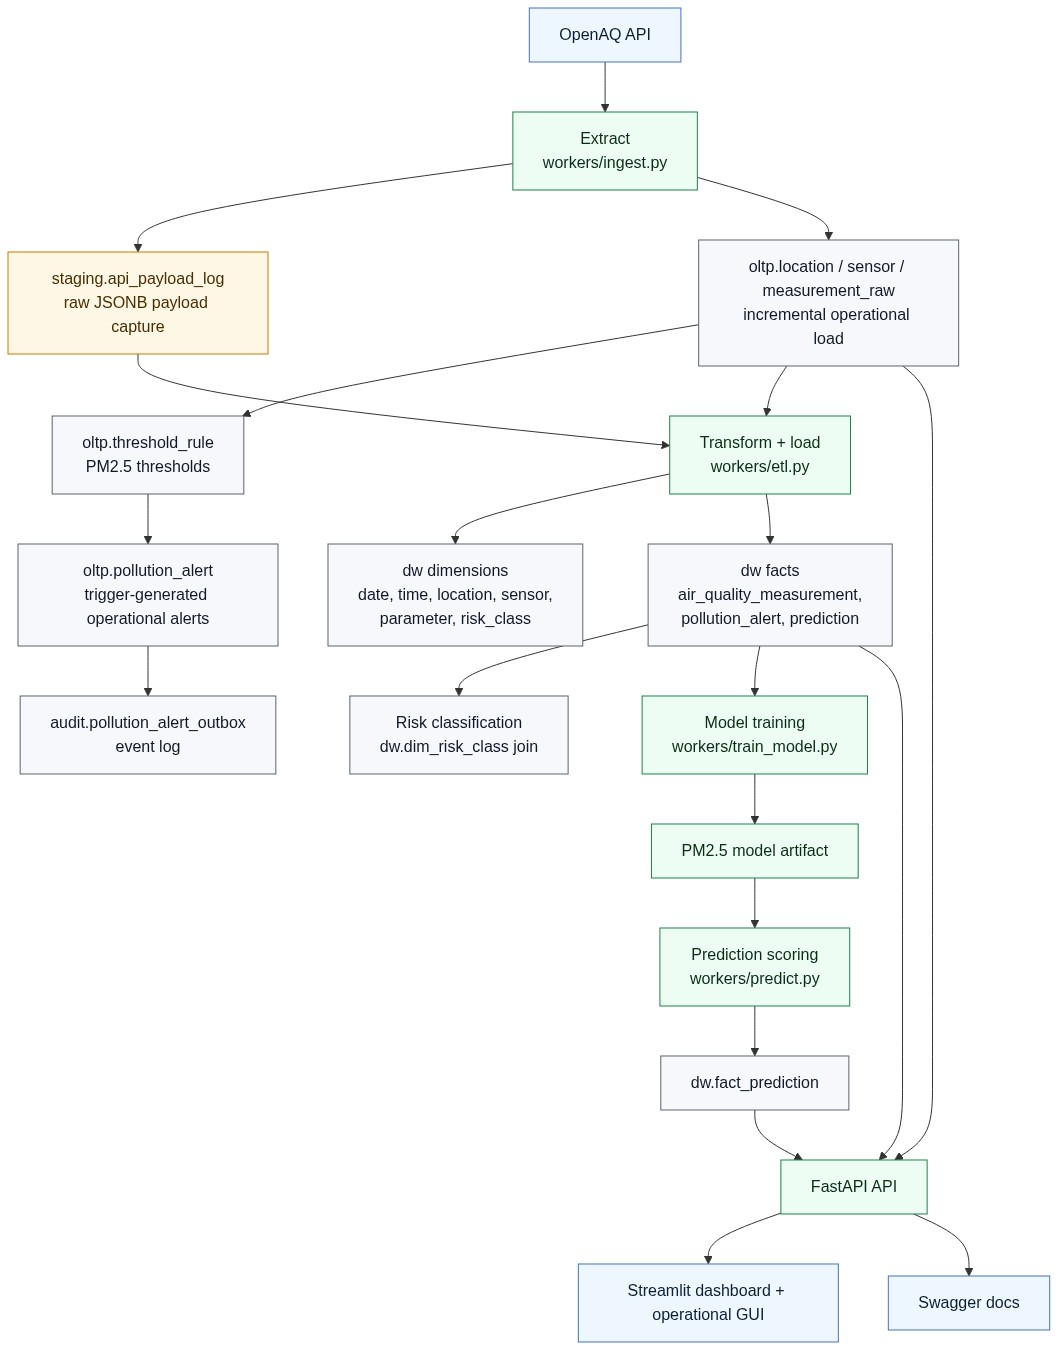
\includegraphics[width=\textwidth]{../../diagrams/data_flow.png}
\caption{End-to-end data flow: source → staging → OLTP → ETL → Data Warehouse → dashboard.}
\label{fig:dataflow}
\end{figure}

% ============================================================
\section{Course Technologies Demonstrated}

The following topics from the Advanced Data Warehouse Technologies course are actively demonstrated:

\subsection{Star Schema Design (Chapter~1)}

The DW uses a \textbf{fact constellation} (galaxy schema): three fact tables sharing conformed dimensions.
This is a standard DW pattern when multiple business processes (measurements, alerts, predictions)
share the same dimensional context (date, time, location, sensor, parameter).

\begin{itemize}[nosep]
  \item \textbf{Conformed dimensions:} \texttt{dim\_date} and \texttt{dim\_time} are pre-populated and shared across all facts.
  \item \textbf{Degenerate dimensions:} measurement unit stored directly on the fact row.
  \item \textbf{Hierarchies:} date dimension supports year → quarter → month → day drill-down.
  \item \textbf{Reference dimension:} \texttt{dim\_risk\_class} maps continuous PM2.5 values to categorical severity bands.
\end{itemize}

\subsection{Slowly Changing Dimensions --- SCD Type~2 (Chapter~2)}

\begin{itemize}[nosep]
  \item \texttt{dim\_location} and \texttt{dim\_sensor} implement \textbf{SCD Type~2} with columns: \texttt{valid\_from}, \texttt{valid\_to}, \texttt{is\_current}.
  \item Change detection uses \textbf{MD5 hash comparison} of attribute values.
  \item When a location changes (e.g., name update, coordinate correction): the current row is expired (\texttt{valid\_to = now, is\_current = false}) and a new row is inserted with a new surrogate key.
  \item Historical queries can join facts to the dimension version that was valid at measurement time.
\end{itemize}

\subsection{ETL Automation (Chapter~3)}

\begin{itemize}[nosep]
  \item \texttt{workers/etl.py} implements a complete ETL pipeline in Python (analogous to SSIS dataflows):
  \begin{enumerate}[nosep]
    \item \textbf{Extract:} watermark-based incremental pull from OLTP (only rows since last ETL run).
    \item \textbf{Transform:} SCD2 hash comparison, date/time key derivation, risk classification lookup.
    \item \textbf{Load:} bulk insert into fact tables; duplicate-safe via ON CONFLICT DO NOTHING (idempotent re-runs).
  \end{enumerate}
  \item Pipeline idempotency: re-running ETL on the same data produces no duplicates.
\end{itemize}

\subsection{Automated Refresh \& Scheduling (Chapter~3 -- SSIS Jobs)}

The pipeline is scheduled via system cron on the production VM:
\begin{itemize}[nosep]
  \item \textbf{Every 3 hours}: \texttt{run\_pipeline.sh ingest-etl} --- fetch new data and load into DW.
  \item \textbf{Daily at 06:00 UTC}: \texttt{run\_pipeline.sh predict-only} --- generate next-period predictions.
  \item \textbf{Weekly Sunday 03:00 UTC}: \texttt{run\_pipeline.sh train-predict} --- retrain ML model and predict.
\end{itemize}

\subsection{Reports, KPIs \& Visualization (Chapter~5 -- PowerBI/Dashboards)}

The Streamlit dashboard provides analytical views from the DW:
\begin{itemize}[nosep]
  \item \textbf{Air Quality Overview} --- daily aggregated trend charts by parameter.
  \item \textbf{High-Risk Periods} --- heatmaps showing hours/days with elevated pollution.
  \item \textbf{Prediction Insights} --- predicted vs. actual comparison with error metrics.
  \item \textbf{KPI cards} on the home page: total measurements, active alerts, prediction accuracy.
\end{itemize}

\subsection{Machine Learning Integration (100\% criterion)}

\begin{itemize}[nosep]
  \item A \textbf{Random Forest} model is trained on historical PM2.5 data from the DW.
  \item Features: current value, lag-1, rolling 3h/6h means, temporal (hour, weekday, month), sensor/location keys.
  \item Predictions are stored as \texttt{fact\_prediction} with associated \texttt{risk\_class\_key}.
  \item Model metrics tracked: MAE, RMSE, R\textsuperscript{2} (currently $R^2 \approx 0.73$).
\end{itemize}

\subsection{DB Administration \& Alerts (Chapter~7)}

\begin{itemize}[nosep]
  \item Threshold-based alerting rules trigger pollution alerts automatically.
  \item Alert lifecycle tracked in DW as \texttt{fact\_pollution\_alert}.
  \item Automated backups (daily \texttt{pg\_dump}) and scheduled maintenance (VACUUM/ANALYZE).
\end{itemize}

% ============================================================
\section{Functional Specification}

\begin{enumerate}[nosep]
  \item \textbf{Data Ingestion} --- Incremental and bulk ingest from OpenAQ v3 API with error tracking.
  \item \textbf{ETL Pipeline} --- Extracts from OLTP, applies SCD2, loads facts incrementally.
  \item \textbf{Star Schema (Fact Constellation)} --- Three fact tables with six shared dimensions.
  \item \textbf{SCD Type~2} --- History-preserving dimensions with hash-based change detection.
  \item \textbf{Risk Classification} --- PM2.5 values classified into Low / Moderate / High / Critical.
  \item \textbf{PM2.5 Prediction} --- Random Forest model; predictions stored in \texttt{fact\_prediction}.
  \item \textbf{Automated Refresh} --- Cron-scheduled pipeline (every 3h ingest-ETL, daily predict).
  \item \textbf{Analytical Dashboard} --- Streamlit with trend charts, heatmaps, KPIs.
  \item \textbf{Threshold Alerts} --- Configurable rules; alerts loaded into DW as facts.
  \item \textbf{Deployment} --- Docker Compose on Hetzner Cloud with automatic HTTPS.
\end{enumerate}

% ============================================================
\section{Logical Data Model (Star Schema)}

\begin{figure}[H]
\centering
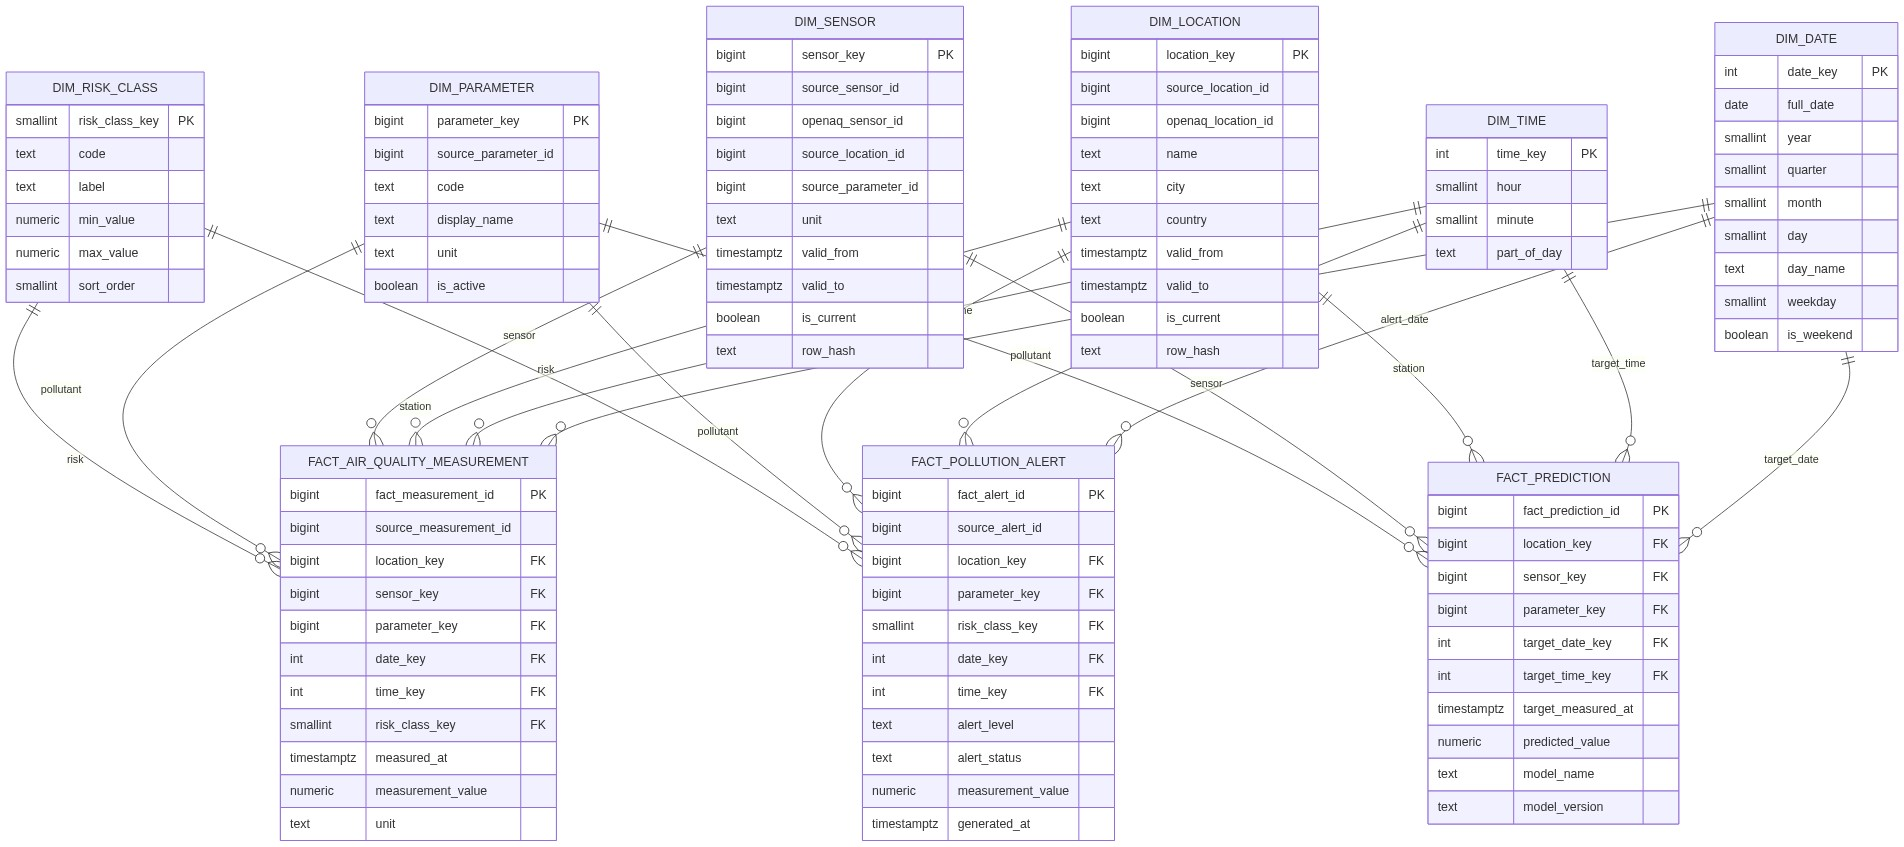
\includegraphics[width=\textwidth]{../../diagrams/dw_star_schema.png}
\caption{Data warehouse star schema (fact constellation with shared dimensions).}
\label{fig:star}
\end{figure}

\subsection*{Fact Tables}

The design uses a \textbf{fact constellation} (also called galaxy schema), where multiple fact tables
share conformed dimensions. This is standard practice when a DW serves multiple related business processes.

\begin{table}[H]
\centering
\small
\begin{tabular}{@{}lll@{}}
\toprule
\textbf{Table} & \textbf{Grain} & \textbf{Measures} \\
\midrule
\texttt{fact\_air\_quality\_measurement} & One reading per sensor per timestamp & \texttt{measurement\_value}, unit \\
\texttt{fact\_pollution\_alert} & One alert event & \texttt{measurement\_value}, level, status \\
\texttt{fact\_prediction} & One prediction per location/time & \texttt{predicted\_value}, model info \\
\bottomrule
\end{tabular}
\caption{Fact tables --- three business processes sharing conformed dimensions.}
\end{table}

\subsection*{Dimension Tables}

\begin{table}[H]
\centering
\small
\begin{tabular}{@{}llp{6.5cm}@{}}
\toprule
\textbf{Table} & \textbf{Type} & \textbf{Description} \\
\midrule
\texttt{dim\_date} & Conformed, pre-populated & Calendar attributes (year, quarter, month, weekday, is\_weekend) \\
\texttt{dim\_time} & Conformed, pre-populated & Hour/minute with part-of-day classification \\
\texttt{dim\_parameter} & Type~1 & Pollutant definitions (pm25, pm10, no2, o3) \\
\texttt{dim\_location} & SCD Type~2 & Monitoring stations with validity range \\
\texttt{dim\_sensor} & SCD Type~2 & Sensors with validity range \\
\texttt{dim\_risk\_class} & Reference & PM2.5 concentration bands (WHO guidelines) \\
\bottomrule
\end{tabular}
\caption{Dimension tables.}
\end{table}

% ============================================================
\section{Technologies Used}

\begin{table}[H]
\centering
\begin{tabular}{@{}ll@{}}
\toprule
\textbf{Technology} & \textbf{Role} \\
\midrule
PostgreSQL 16 & OLTP + Data Warehouse (schema separation) \\
Python 3.12 & ETL scripts, ML training, prediction, ingestion \\
scikit-learn & Random Forest model for PM2.5 prediction \\
pandas & Data transformation and feature engineering \\
Streamlit & Analytical multi-page dashboard \\
Plotly & Interactive charts (line, bar, heatmap) \\
FastAPI & REST API serving DW data \\
Docker Compose & Service orchestration (5 containers) \\
Caddy 2 & HTTPS reverse proxy (Let's Encrypt) \\
GitHub Actions & CI/CD deployment pipeline \\
Hetzner Cloud & Production VM (Ubuntu 24.04) \\
\bottomrule
\end{tabular}
\end{table}

\end{document}
